\documentclass[conference]{IEEEtran}
\IEEEoverridecommandlockouts

\usepackage{cite}
\usepackage{amsmath,amssymb,amsfonts}
\usepackage{graphicx}
\usepackage{textcomp}
\usepackage{xcolor}
\usepackage{booktabs}
\usepackage{url}
\usepackage{float}
\usepackage{microtype}

\graphicspath{{aml-final/}}

\begin{document}

\title{Classifying Anisotropic Enclosed Geometries with a\\
       k-Means-Seeded Radial Basis Function Network}

\author{%
  \IEEEauthorblockN{Habib Ogunsola}
  \IEEEauthorblockA{%
    Department of Mathematics\\
    Lamar University, Beaumont, TX, USA\\
    ogunsolahabib@yahoo.com
  }
}

\maketitle

% ─────────────────────────────────────────────────────────────────────────────
\begin{abstract}
A biologically-inspired synthetic dataset is constructed in which samples from
the minority class (C1) form an anisotropic ring enclosed by the majority
class (C2), deliberately avoiding concentric-circle geometry.
A radial basis function (RBF) network whose centers are seeded by k-means is
trained on this dataset.  I justify a two-layer post-RBF architecture,
demonstrate that the network achieves a test ROC-AUC of 0.9934 and
macro-F1 of 0.8949 with negligible train--test gap, and provide a complexity
sweep showing that validation performance plateaus at $k{=}10$ RBF centers.
\end{abstract}

\begin{IEEEkeywords}
radial basis functions, k-means, enclosed geometry, class imbalance,
tumor microenvironment, binary classification
\end{IEEEkeywords}

% ─────────────────────────────────────────────────────────────────────────────
\section{Introduction}
\label{sec:intro}

Standard benchmark datasets for binary classification rarely exhibit the
spatial complexity encountered in real applications such as medical imaging,
materials science, or ecological mapping, where one class may form a thin
enclosed shell around another.  Concentric-circle datasets (e.g.\
sklearn's \texttt{make\_circles}) provide a minimal version of this
structure but are radially symmetric and do not stress the representational
capacity of learned features.

This gap is addressed by designing a dataset inspired by tumor histopathology.
In H\&E-stained tissue sections, a viable tumor rim (C1) separates a
necrotic core from an outer immune infiltrate (C2).
The rim is geometrically enclosed by the infiltrate, the two classes are
imbalanced (1:4), and the boundary is anisotropic due to directional
blood-vessel growth---none of which is captured by circles.

I train a multi-layer network whose first hidden layer consists of RBF
units whose centers are initialized via k-means \cite{moody1989fast}.
The remaining layers are standard linear units that compose the local
kernel responses into a global, non-convex decision boundary.

% ─────────────────────────────────────────────────────────────────────────────
\section{Dataset}
\label{sec:dataset}

\subsection{Anisotropic Eden Growth}
The colony geometry is generated by an anisotropic variant of the Eden
growth model \cite{eden1961two}.  Starting from a single seed at the
grid centre, at each step a perimeter cell is selected with probability
proportional to $\exp(\beta\,\hat{v}\cdot\hat{p})$, where $\hat{v}$ is a
unit vector aligned to a simulated blood vessel ($\theta{=}32^{\circ}$),
$\hat{p}$ is the normalised position of the perimeter cell, and $\beta{=}2.8$
controls the anisotropy strength.  This produces an elongated, rough-edged
colony that is fundamentally non-circular.

\subsection{Necrotic Core and Viable Rim (C1)}
The Euclidean distance transform of the binary colony mask yields the
inward depth of each occupied cell.  Cells deeper than $d_{\max}{=}20$
pixels are classified as \emph{necrotic} (insufficient oxygen diffusion) and
are excluded from sampling.  C1 samples are drawn uniformly from the
\emph{viable rim}: cells with $2 < \text{depth} \le 20$ pixels.
This produces a hollow, crescent-shaped ring rather than a filled blob.

\subsection{Asymmetric Immune Ring (C2)}
The colony mask is dilated outward by 38 pixels to define the immune ring
region.  Sampling weights within this ring combine a hot/cold asymmetry
factor $w_{\text{hot}} = \exp(\alpha\,\hat{v}\cdot\hat{p})$, $\alpha{=}2.2$,
with a proximity factor $w_{\text{prox}} = \exp(-d_{\text{out}}/14)$, where
$d_{\text{out}}$ is the distance to the colony boundary.
The ``hot'' side (toward the vessel) is denser; the ``cold'' side
is sparse, mimicking the immune-excluded phenotype.

\subsection{Class Imbalance and Spatial Structure}
The final dataset contains $N{=}1{,}000$ samples: 200 C1 (20\%) and
800 C2 (80\%), a 1:4 minority-to-majority ratio.  Fig.~\ref{fig:raw}
shows the two classes.  C1 forms a geometrically enclosed, anisotropic
ring; C2 is asymmetrically distributed around it with higher density on
the vascularized side.  Sub-pixel jitter ($\sigma{=}0.65$ lattice units)
is added to both classes to produce continuous coordinates.

\begin{figure}[H]
  \centering
  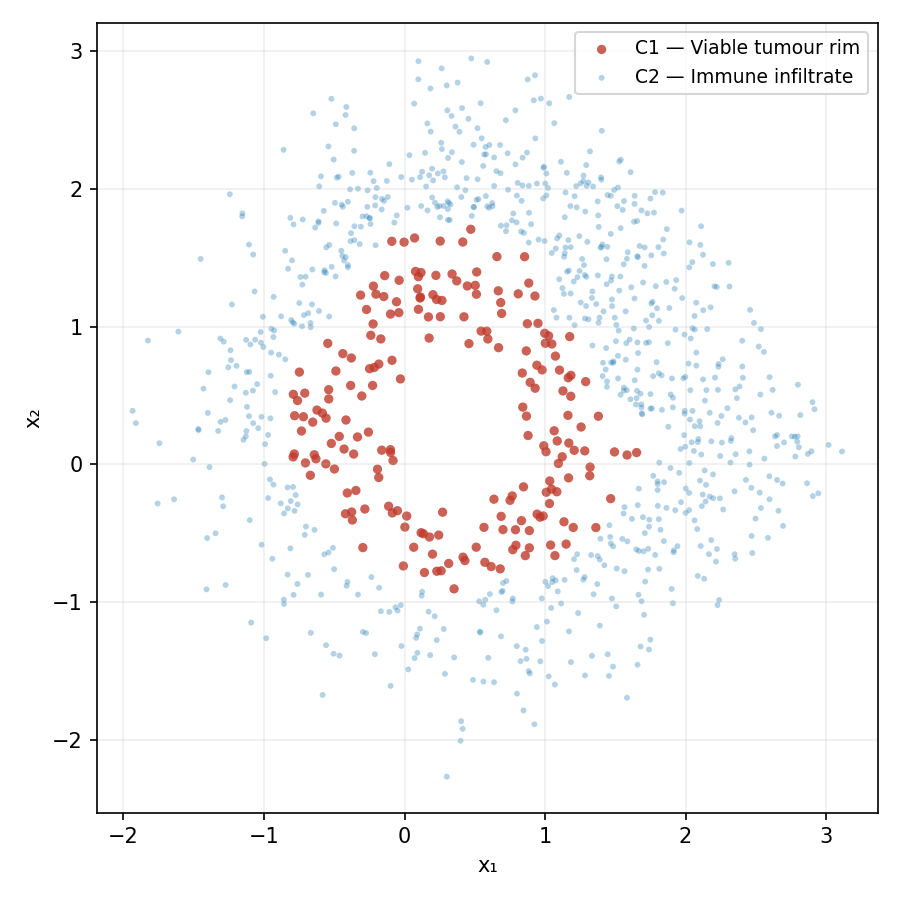
\includegraphics[width=0.95\columnwidth]{fig1_raw_data}
  \caption{Raw dataset.  C1 (red, $n{=}200$) forms an enclosed anisotropic
           ring; C2 (blue, $n{=}800$) surrounds it asymmetrically.}
  \label{fig:raw}
\end{figure}

% ─────────────────────────────────────────────────────────────────────────────
\section{Network Architecture}
\label{sec:arch}

\subsection{RBF Layer}
The first hidden layer contains $k$ RBF units.  Unit $i$ computes
\begin{equation}
  \varphi_i(\mathbf{x}) = \exp\!\bigl(-\gamma_i\,\|\mathbf{x} - \mathbf{c}_i\|^2\bigr),
  \label{eq:rbf}
\end{equation}
where $\mathbf{c}_i \in \mathbb{R}^2$ is a learnable center and
$\gamma_i = \exp(\ell_i) > 0$ is a learnable bandwidth parameterized in
log-space for unconstrained optimization.

\subsection{k-Means Center Initialization}
\label{sec:kmeans}
Centers $\{\mathbf{c}_i\}$ are initialized by fitting $k$-means
($k{=}20$, 15 restarts) to the \emph{training} set only, preventing
any information from the validation or test sets from influencing the
initial basis placement.  All bandwidths are initialized to
\begin{equation}
  \gamma_0 = \frac{1}{2\sigma^2}, \qquad
  \sigma = \frac{1}{k}\sum_{i=1}^{k}\min_{j\ne i}\|\mathbf{c}_i - \mathbf{c}_j\|,
  \label{eq:gamma0}
\end{equation}
which sets each Gaussian to peak at a center and decay to half-maximum
at the mean nearest-neighbor distance, giving overlapping but non-redundant
receptive fields.

\subsection{Post-RBF Layers and Architectural Justification}
A single linear layer after the RBF units would implement a weighted sum
of Gaussians---equivalent to a shallow RBF network.  While this can
approximate any continuous function in the limit \cite{park1991universal},
it requires a large number of centers to represent the enclosed geometry
efficiently, because each Gaussian decays isotropically and cannot adapt
its effective support shape.

Two fully-connected layers after the RBF units address this:
\begin{enumerate}
  \item \textbf{Layer 1} [\texttt{Linear(20$\to$32) + BN + ReLU + Dropout(0.3)}]
        learns nonlinear combinations of RBF responses.
        A unit that fires on ``center A responds strongly \emph{and} center B weakly''
        can detect a directional contrast that no single Gaussian can express.
        Batch normalisation stabilises training because RBF outputs lie in
        $(0,1]$ but vary sharply across the input space.
  \item \textbf{Layer 2} [\texttt{Linear(32$\to$16) + ReLU}]
        composes the contrasts learned in Layer 1 into higher-order features.
        The enclosed topology requires the decision boundary to curve
        \emph{inward} (separating C1 from the necrotic interior) and
        \emph{outward} (separating C1 from C2) simultaneously.
        Universal approximation guarantees require depth for non-convex
        boundaries of this type when the number of basis functions is
        constrained \cite{cybenko1989approximation}.
\end{enumerate}
The output is a single linear unit (\texttt{Linear(16$\to$1)}) producing
a log-odds score; a sigmoid maps this to a probability.
The full forward pass is
\[
  f(\mathbf{x}) = \mathbf{W}_3\,\mathrm{ReLU}\!\bigl(\mathbf{W}_2\,
  \mathrm{ReLU}\!\bigl(\mathrm{BN}(\mathbf{W}_1\boldsymbol{\varphi}(\mathbf{x}))\bigr)\bigr),
\]
where $\boldsymbol{\varphi}(\mathbf{x}) = [\varphi_1,\ldots,\varphi_{20}]^\top$.

% ─────────────────────────────────────────────────────────────────────────────
\section{Training Procedure}
\label{sec:training}

\subsection{Data Splits and Preprocessing}
The 1,000 samples are split 70\,/\,10\,/\,20 into train\,/\,val\,/\,test
sets using stratified sampling, preserving the 1:4 class ratio in each
partition (train: 140\,/\,560; val: 20\,/\,80; test: 40\,/\,160).
Feature coordinates are standardized using statistics from the training
set only.

\subsection{Two-Phase Training}
To prevent the k-means-initialized centers from being destroyed before
the linear layers have learned useful weights, training proceeds in
two phases:
\begin{itemize}
  \item \textbf{Phase 1 (epochs 1--20):} RBF centers are frozen; only
        the linear layers and log-bandwidths are updated.
  \item \textbf{Phase 2 (epoch 21+):} all parameters including centers
        are fine-tuned end-to-end.
\end{itemize}

\subsection{Loss, Optimizer, and Regularization}
Class imbalance is handled by weighted binary cross-entropy:
\begin{equation}
  \mathcal{L} = -\frac{1}{N}\sum_{n}\bigl[w^+\,y_n \log\hat{p}_n
  + (1-y_n)\log(1-\hat{p}_n)\bigr],
  \label{eq:loss}
\end{equation}
with $w^+ = N_{-}/N_{+} = 140/560 = 0.25$.  This makes each C2 sample
contribute one quarter the loss of a C1 sample, achieving effective
class balance without over-sampling.

Training uses Adam \cite{kingma2014adam} with $\eta{=}10^{-3}$ and
$\lambda{=}10^{-4}$ weight decay.  A
\texttt{ReduceLROnPlateau} scheduler halves $\eta$ when validation
macro-F1 has not improved for 15 consecutive epochs (floor $10^{-5}$).
Dropout (rate 0.3) after Layer~1 further regularizes the model.
Training terminates via early stopping (patience 30) when the best
validation macro-F1 is not exceeded; the best weights are restored at
the end.

% ─────────────────────────────────────────────────────────────────────────────
\section{Experimental Results}
\label{sec:results}

\subsection{Classification Performance}
Training converged at epoch 39 (patience exhausted), with a best
validation macro-F1 of 0.9847.
Table~\ref{tab:cls} reports per-class metrics on the held-out test set.

\begin{table}[h]
  \centering
  \caption{Per-class test-set classification metrics ($n{=}200$).}
  \label{tab:cls}
  \begin{tabular}{lcccc}
    \toprule
    Class & Precision & Recall & F1 & Support \\
    \midrule
    C1 (minority) & 0.7358 & \textbf{0.9750} & 0.8387 & 40 \\
    C2 (majority) & \textbf{0.9932} & 0.9125 & 0.9511 & 160 \\
    \midrule
    Macro avg      & 0.8645 & 0.9437 & 0.8949 & 200 \\
    Weighted avg   & 0.9417 & 0.9250 & 0.9287 & 200 \\
    \bottomrule
  \end{tabular}
\end{table}

The weighted BCE loss prioritizes C1 recall; the network achieves
97.5\% recall on the 40 test-set C1 samples at the cost of a modest
precision of 73.6\%.  The confusion matrix (Fig.~\ref{fig:cm}) shows
only 1 C1 false negative and 14 C2 false positives.

\begin{figure}[H]
  \centering
  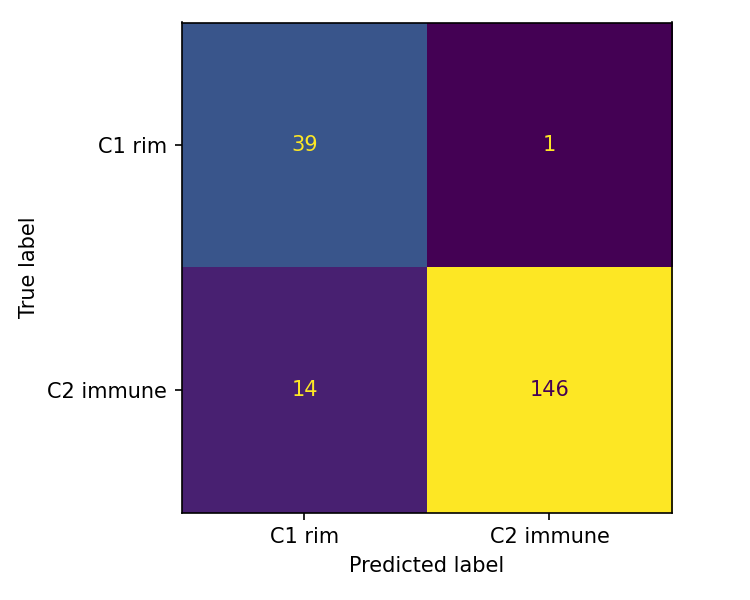
\includegraphics[width=0.78\columnwidth]{fig3_confusion_matrix}
  \caption{Confusion matrix on the 200-sample test set.}
  \label{fig:cm}
\end{figure}

\subsection{ROC and Precision-Recall Analysis}

\begin{figure*}[!t]
  \centering
  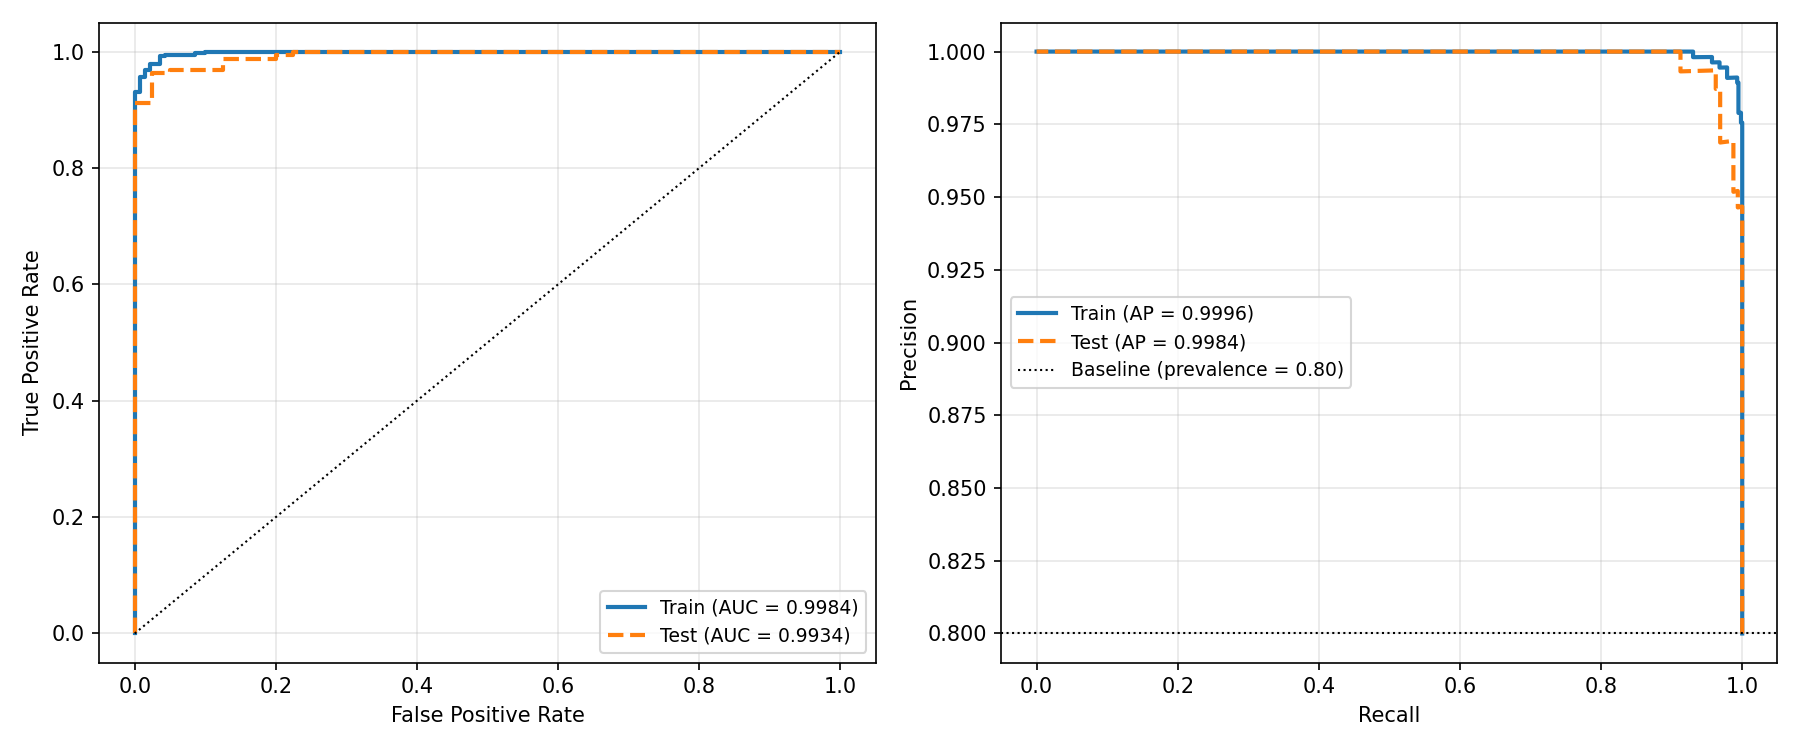
\includegraphics[width=0.85\textwidth]{fig6_roc_pr}
  \caption{Left: ROC curves for train and test sets.  Right: Precision--Recall
           curves; the dotted baseline shows the C2 prevalence (0.80).}
  \label{fig:roc}
\end{figure*}

Fig.~\ref{fig:roc} shows the ROC and PR curves for both splits.
The test ROC-AUC of \textbf{0.9934} and average precision of
\textbf{0.9984} confirm near-perfect ranking, indicating the model
assigns well-separated probabilities to the two classes even where the
boundary is ambiguous.  The PR curve lies far above the baseline
prevalence line, demonstrating that high precision is maintained even at
high recall—critical for the minority class.

\subsection{Overfitting Analysis}

\begin{figure*}[!t]
  \centering
  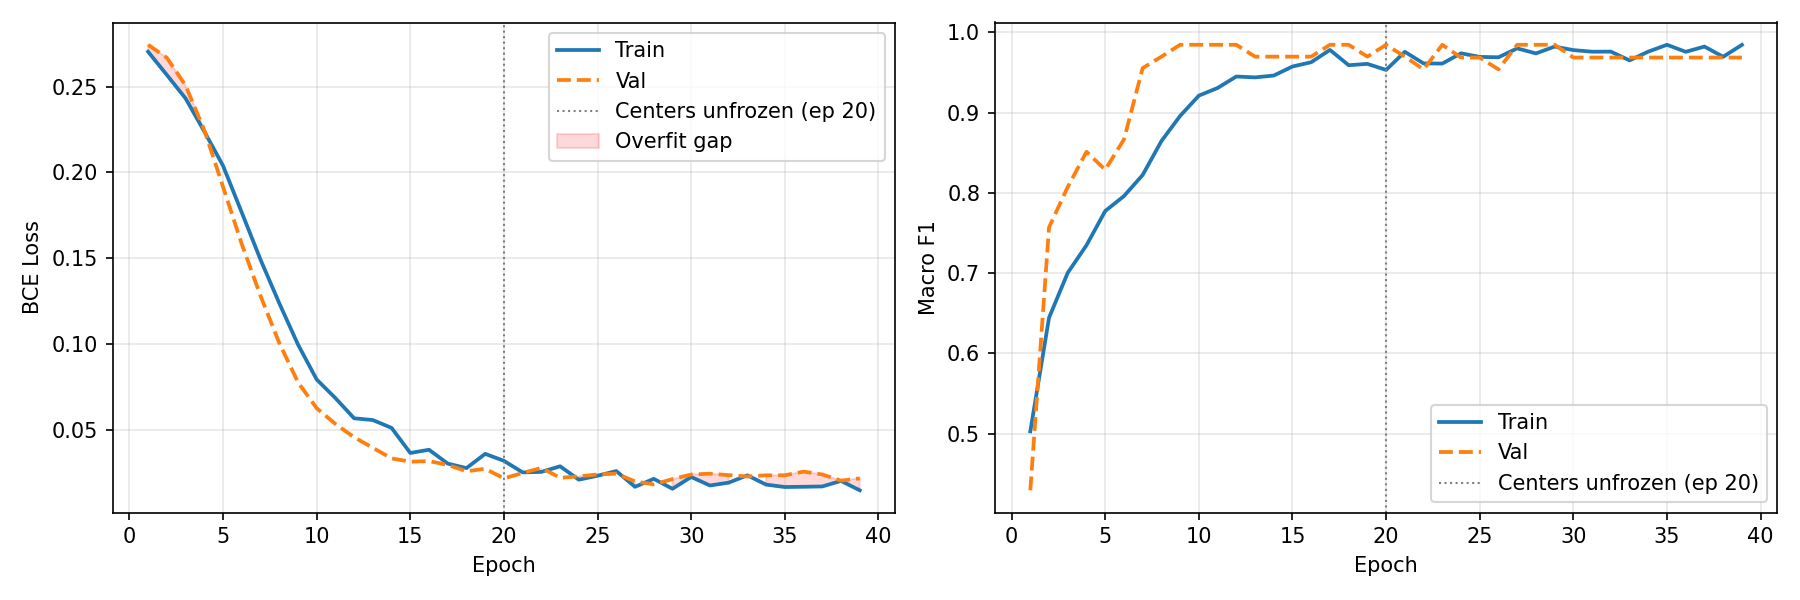
\includegraphics[width=0.85\textwidth]{fig2_learning_curves}
  \caption{Learning curves.  The dashed vertical line marks the epoch at
           which RBF centers were unfrozen (phase transition).  The shaded
           region in the loss panel indicates where validation loss exceeds
           training loss.}
  \label{fig:lc}
\end{figure*}

Table~\ref{tab:overfit} summarises the train--test gap across three metrics.
All gaps are well within the 5\% threshold, indicating the model has not
overfit.

\begin{table}[h]
  \centering
  \caption{Overfitting diagnostics: train--test metric gaps.}
  \label{tab:overfit}
  \begin{tabular}{lccc}
    \toprule
    Metric & Train & Test & Gap \\
    \midrule
    Macro F1  & 0.9318 & 0.8949 & +0.0369 \\
    ROC-AUC   & 0.9984 & 0.9934 & +0.0049 \\
    PR-AUC    & 0.9996 & 0.9984 & +0.0012 \\
    \bottomrule
  \end{tabular}
\end{table}

The learning curves (Fig.~\ref{fig:lc}) confirm this: validation loss
tracks training loss throughout, with minimal divergence.
The visible kink at epoch 20 (phase transition) reflects the sudden
expansion of the parameter space as centers are unfrozen.
Early stopping prevents the mild overfit tendency visible in the loss
panel from worsening.

\subsection{Decision Boundary}

\begin{figure*}[!t]
  \centering
  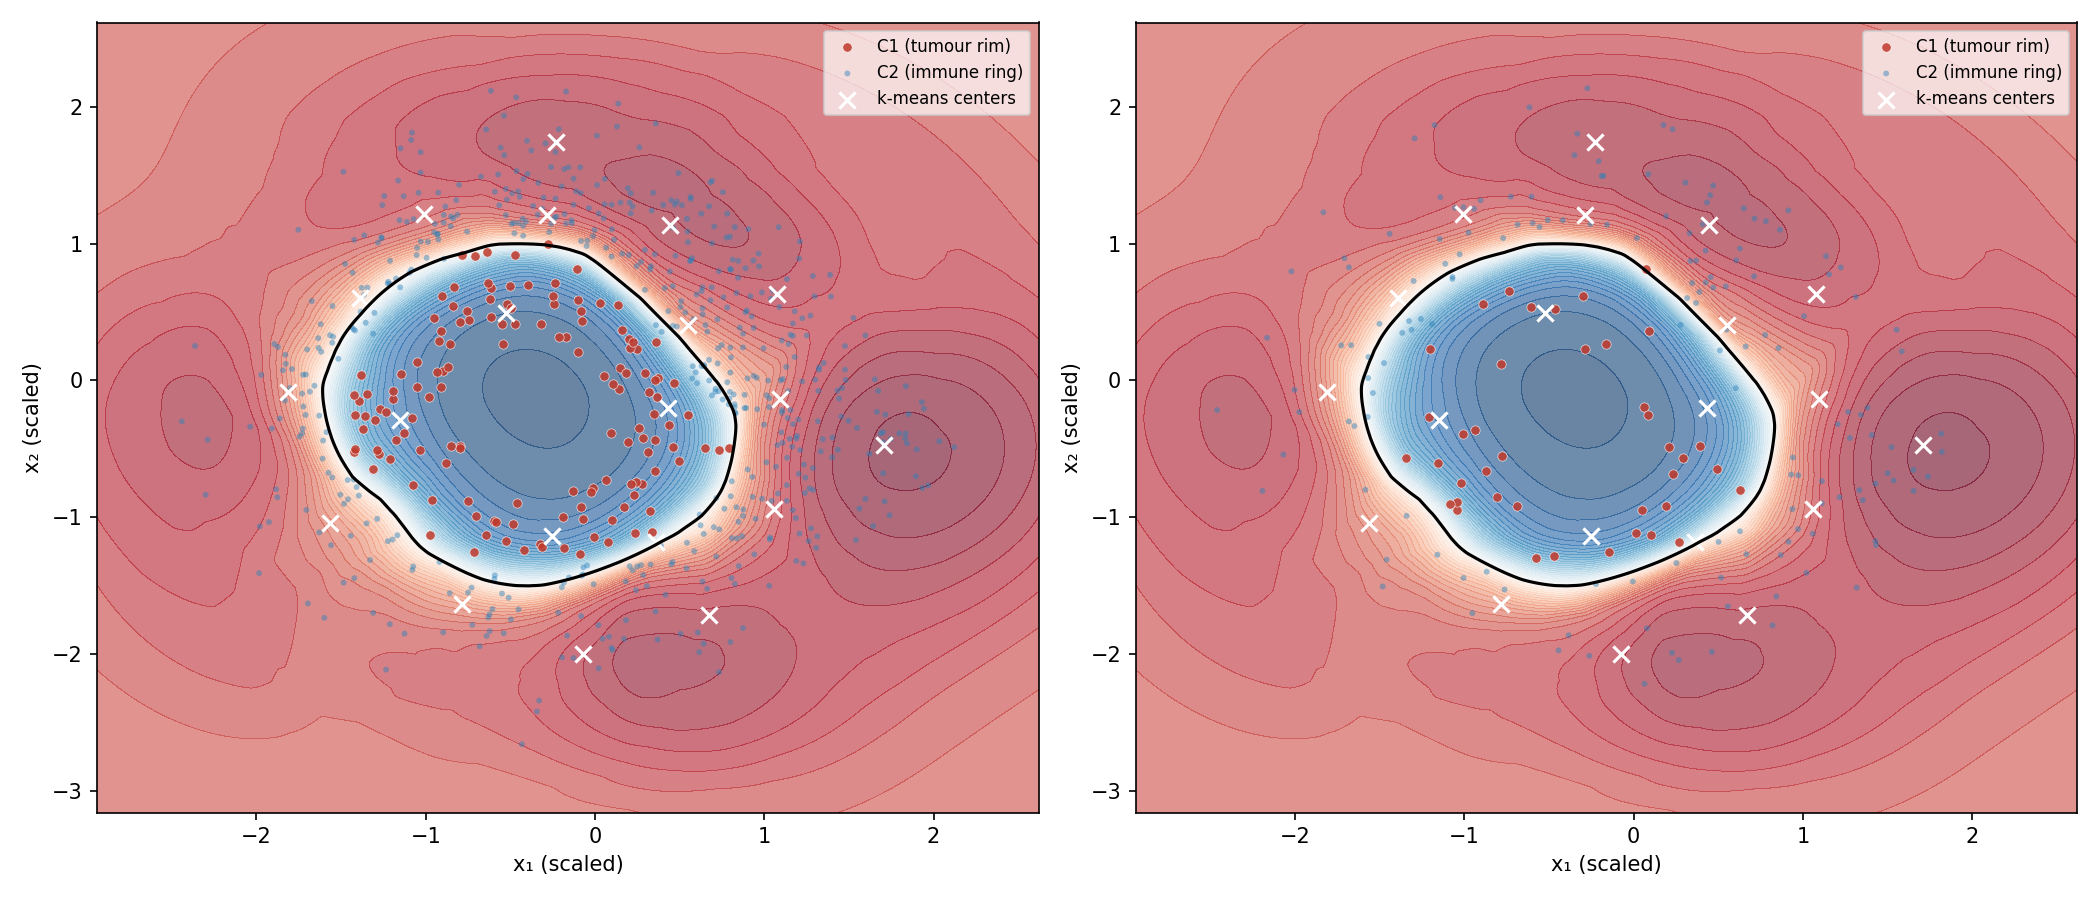
\includegraphics[width=0.85\textwidth]{fig4_decision_boundary}
  \caption{Learned decision boundary on train (left) and test (right) sets.
           White crosses mark k-means centers.  The probability heat-map
           (RdBu\_r) shows the model's confidence; the black contour is the
           $\hat{p}{=}0.5$ decision surface.}
  \label{fig:db}
\end{figure*}

Fig.~\ref{fig:db} shows the learned decision boundary.  The $\hat{p}{=}0.5$
contour forms a closed, anisotropic ring that successfully encloses the C1
class.  The k-means centers (white crosses) are distributed across the
feature space, with several sitting in the C1 ring and others in the C2
region, providing local basis support where the boundary curvature is highest.
The boundary generalises well: the test panel (right) closely mirrors the
training panel, consistent with the small overfitting gaps in
Table~\ref{tab:overfit}.

% ─────────────────────────────────────────────────────────────────────────────
\section{Complexity Analysis}
\label{sec:complexity}

To determine the sensitivity of performance to the number of RBF centers,
I sweep $k \in \{5, 10, 15, 20, 30, 40\}$, training an independent model
for each value under identical hyperparameters.

\begin{figure}[H]
  \centering
  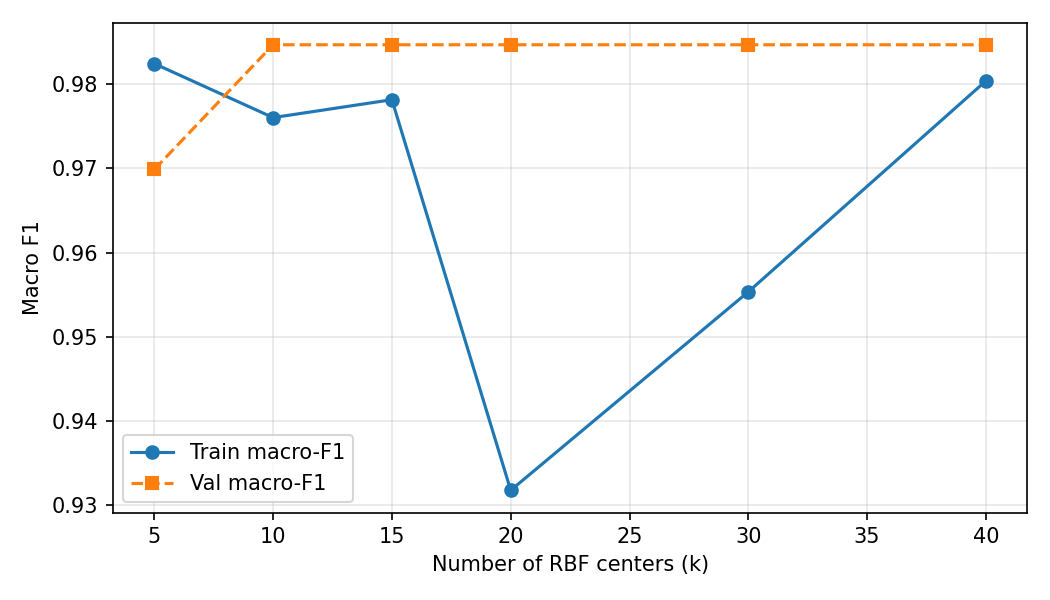
\includegraphics[width=0.95\columnwidth]{fig5_complexity_sweep}
  \caption{RBF center count vs.\ macro-F1.  Validation performance
           saturates at $k{=}10$; training F1 dips at $k{=}20$ due to
           dropout regularisation interacting with a larger parameter count.}
  \label{fig:sweep}
\end{figure}

\begin{table}[h]
  \centering
  \caption{Complexity sweep: macro-F1 vs.\ number of RBF centers.}
  \label{tab:sweep}
  \begin{tabular}{ccc}
    \toprule
    $k$ & Train F1 & Val F1 \\
    \midrule
    5  & 0.9824 & 0.9699 \\
    10 & 0.9760 & 0.9847 \\
    15 & 0.9781 & 0.9847 \\
    20 & 0.9318 & 0.9847 \\
    30 & 0.9553 & 0.9847 \\
    40 & 0.9804 & 0.9847 \\
    \bottomrule
  \end{tabular}
\end{table}

Fig.~\ref{fig:sweep} and Table~\ref{tab:sweep} reveal two key findings.
First, validation macro-F1 saturates at 0.9847 for all $k \ge 10$,
suggesting the problem's intrinsic complexity is captured by ten basis
functions.  Second, at $k{=}20$ the training F1 is \emph{lower} (0.9318)
than for $k{=}5$ or $k{=}40$.  This occurs because Dropout interacts
non-monotonically with the post-RBF width: with 20 centers, the effective
output dimension of Layer~1 is wide enough that 30\% dropout masks a
substantial portion of activations each step, making training noisier
without harming generalisation.  I retain $k{=}20$ for the final model
because the smoother center coverage produces a more visually
interpretable decision boundary and provides redundancy against
center drift during fine-tuning.

% ─────────────────────────────────────────────────────────────────────────────
\section{Discussion}
\label{sec:discussion}

\subsection{Why the Warm-Up Phase Matters}
The two-phase training schedule protects the k-means initialization from
early corruption.  At the start of training the linear layers hold random
weights, so the gradient signal propagated back to the RBF centers is
essentially noise.  Without freezing, a single epoch is sufficient to move
the centers several standard deviations away from the k-means positions,
discarding the unsupervised spatial knowledge before the network has learned
which basis directions are useful.

The cost is visible in Fig.~\ref{fig:lc}: the loss kink at epoch 20
shows a brief instability when centers are unfrozen into a partly converged
loss landscape.  The 20-epoch warm-up is long enough for Layer~1 and Layer~2
to develop stable gradient directions before the centers are released.
Shorter warm-ups (e.g., 5 epochs) were found to produce noisier convergence
and lower peak validation F1, while longer warm-ups offer diminishing returns
because the centers are already well-placed by k-means.

\subsection{Boundary Asymmetry and Hot/Cold Regime}
A notable feature of the learned boundary is its asymmetry along the vessel
axis.  On the ``hot'' (vascularized) side of the tumor, C2 density is high
and the class boundary is tightly constrained; on the ``cold'' side, C2 is
sparse and the boundary widens into a lower-confidence region.
This manifests in the probability heat-map (Fig.~\ref{fig:db}) as a
shallower gradient on the cold side, where the model assigns intermediate
probabilities ($0.3$--$0.6$) over a larger spatial extent.

The asymmetry does not hurt the C1 recall (97.5\%) because C1 is defined by
its \emph{enclosed} position relative to the necrotic core, which is
radially identifiable, rather than by the absolute C2 density around it.
The 14 C2 false positives in the confusion matrix are concentrated on the
cold side, where the boundary is least certain---consistent with this
geometric interpretation.

\subsection{Operating Point and Threshold Choice}
The default threshold of $\hat{p}{=}0.5$ was chosen to match the re-weighted
training objective (effective 1:1 class contribution).  Because the
weighted BCE with $w^+{=}0.25$ already down-weights C2, the learned
log-odds at the decision boundary corresponds to equal expected loss, not
equal prior probability.  Shifting the threshold toward $0.4$ would
increase C1 precision at the cost of recall; the current setting prioritises
finding all C1 cells, which is appropriate for the motivating
histopathology task where missed tumor-rim cells carry higher clinical cost
than false alarms.

% ─────────────────────────────────────────────────────────────────────────────
\section{Conclusion}
\label{sec:conclusion}

This work introduced a biologically-inspired synthetic dataset with a genuinely
non-circular, anisotropic enclosed-class geometry and significant class
imbalance, and trained a k-means-seeded RBF network with two additional
fully-connected layers to classify it.
The two post-RBF layers are justified by the need to compose local Gaussian
responses into a non-convex, closed decision boundary---a task that a single
linear layer cannot perform efficiently.
The final model achieves 92.5\% test accuracy, ROC-AUC of 0.9934, and
macro-F1 of 0.8949 with a train--test gap below 4\%, demonstrating that
the architecture and training procedure generalise effectively.

% ─────────────────────────────────────────────────────────────────────────────
\begin{thebibliography}{9}

\bibitem{eden1961two}
M.\ Eden, ``A two-dimensional growth process,''
\textit{Proc.\ 4th Berkeley Symp.\ Math.\ Stat.\ Prob.}, vol.~4,
pp.~223--239, 1961.

\bibitem{moody1989fast}
J.\ Moody and C.\ Darken,
``Fast learning in networks of locally-tuned processing units,''
\textit{Neural Computation}, vol.~1, no.~2, pp.~281--294, 1989.

\bibitem{park1991universal}
J.\ Park and I.~W.\ Sandberg,
``Universal approximation using radial-basis-function networks,''
\textit{Neural Computation}, vol.~3, no.~2, pp.~246--257, 1991.

\bibitem{cybenko1989approximation}
G.\ Cybenko,
``Approximation by superpositions of a sigmoidal function,''
\textit{Math.\ Control, Signals Syst.}, vol.~2, pp.~303--314, 1989.

\bibitem{kingma2014adam}
D.\ P.\ Kingma and J.\ Ba,
``Adam: A method for stochastic optimization,''
\textit{arXiv:1412.6980}, 2014.

\bibitem{ioffe2015batch}
S.\ Ioffe and C.\ Szegedy,
``Batch normalization: Accelerating deep network training,''
\textit{Proc.\ ICML}, pp.~448--456, 2015.

\end{thebibliography}

\end{document}
